\subsubsection{朴素IVF算法多线程}

本节对朴素IVF算法的多线程实现进行深入分析,主要比较了串行实现、OpenMP并行实现和Pthread并行实现在不同参数配置下的性能表现。

\paragraph{实验设置}

我们在相同的硬件环境下测试了三种不同的IVF算法实现:
\begin{itemize}
    \item \textbf{串行实现(Serial)}:单线程的基准实现
    \item \textbf{OpenMP实现}:使用OpenMP进行并行优化的版本
    \item \textbf{Pthread实现}:使用Pthread进行多线程优化的版本
\end{itemize}

测试参数范围:
\begin{itemize}
    \item \textbf{nlist}:$\{64, 128, 256, 512\}$ - 聚类中心数量
    \item \textbf{nprobe}:$\{4, 8, 12, 16, 20, 24, 32\}$ - 搜索的聚类数量
\end{itemize}

\paragraph{性能分析结果}

图~\ref{fig:ivf_comprehensive}展示了IVF算法多线程实现的综合性能分析。

\begin{figure}[htbp]
    \centering
    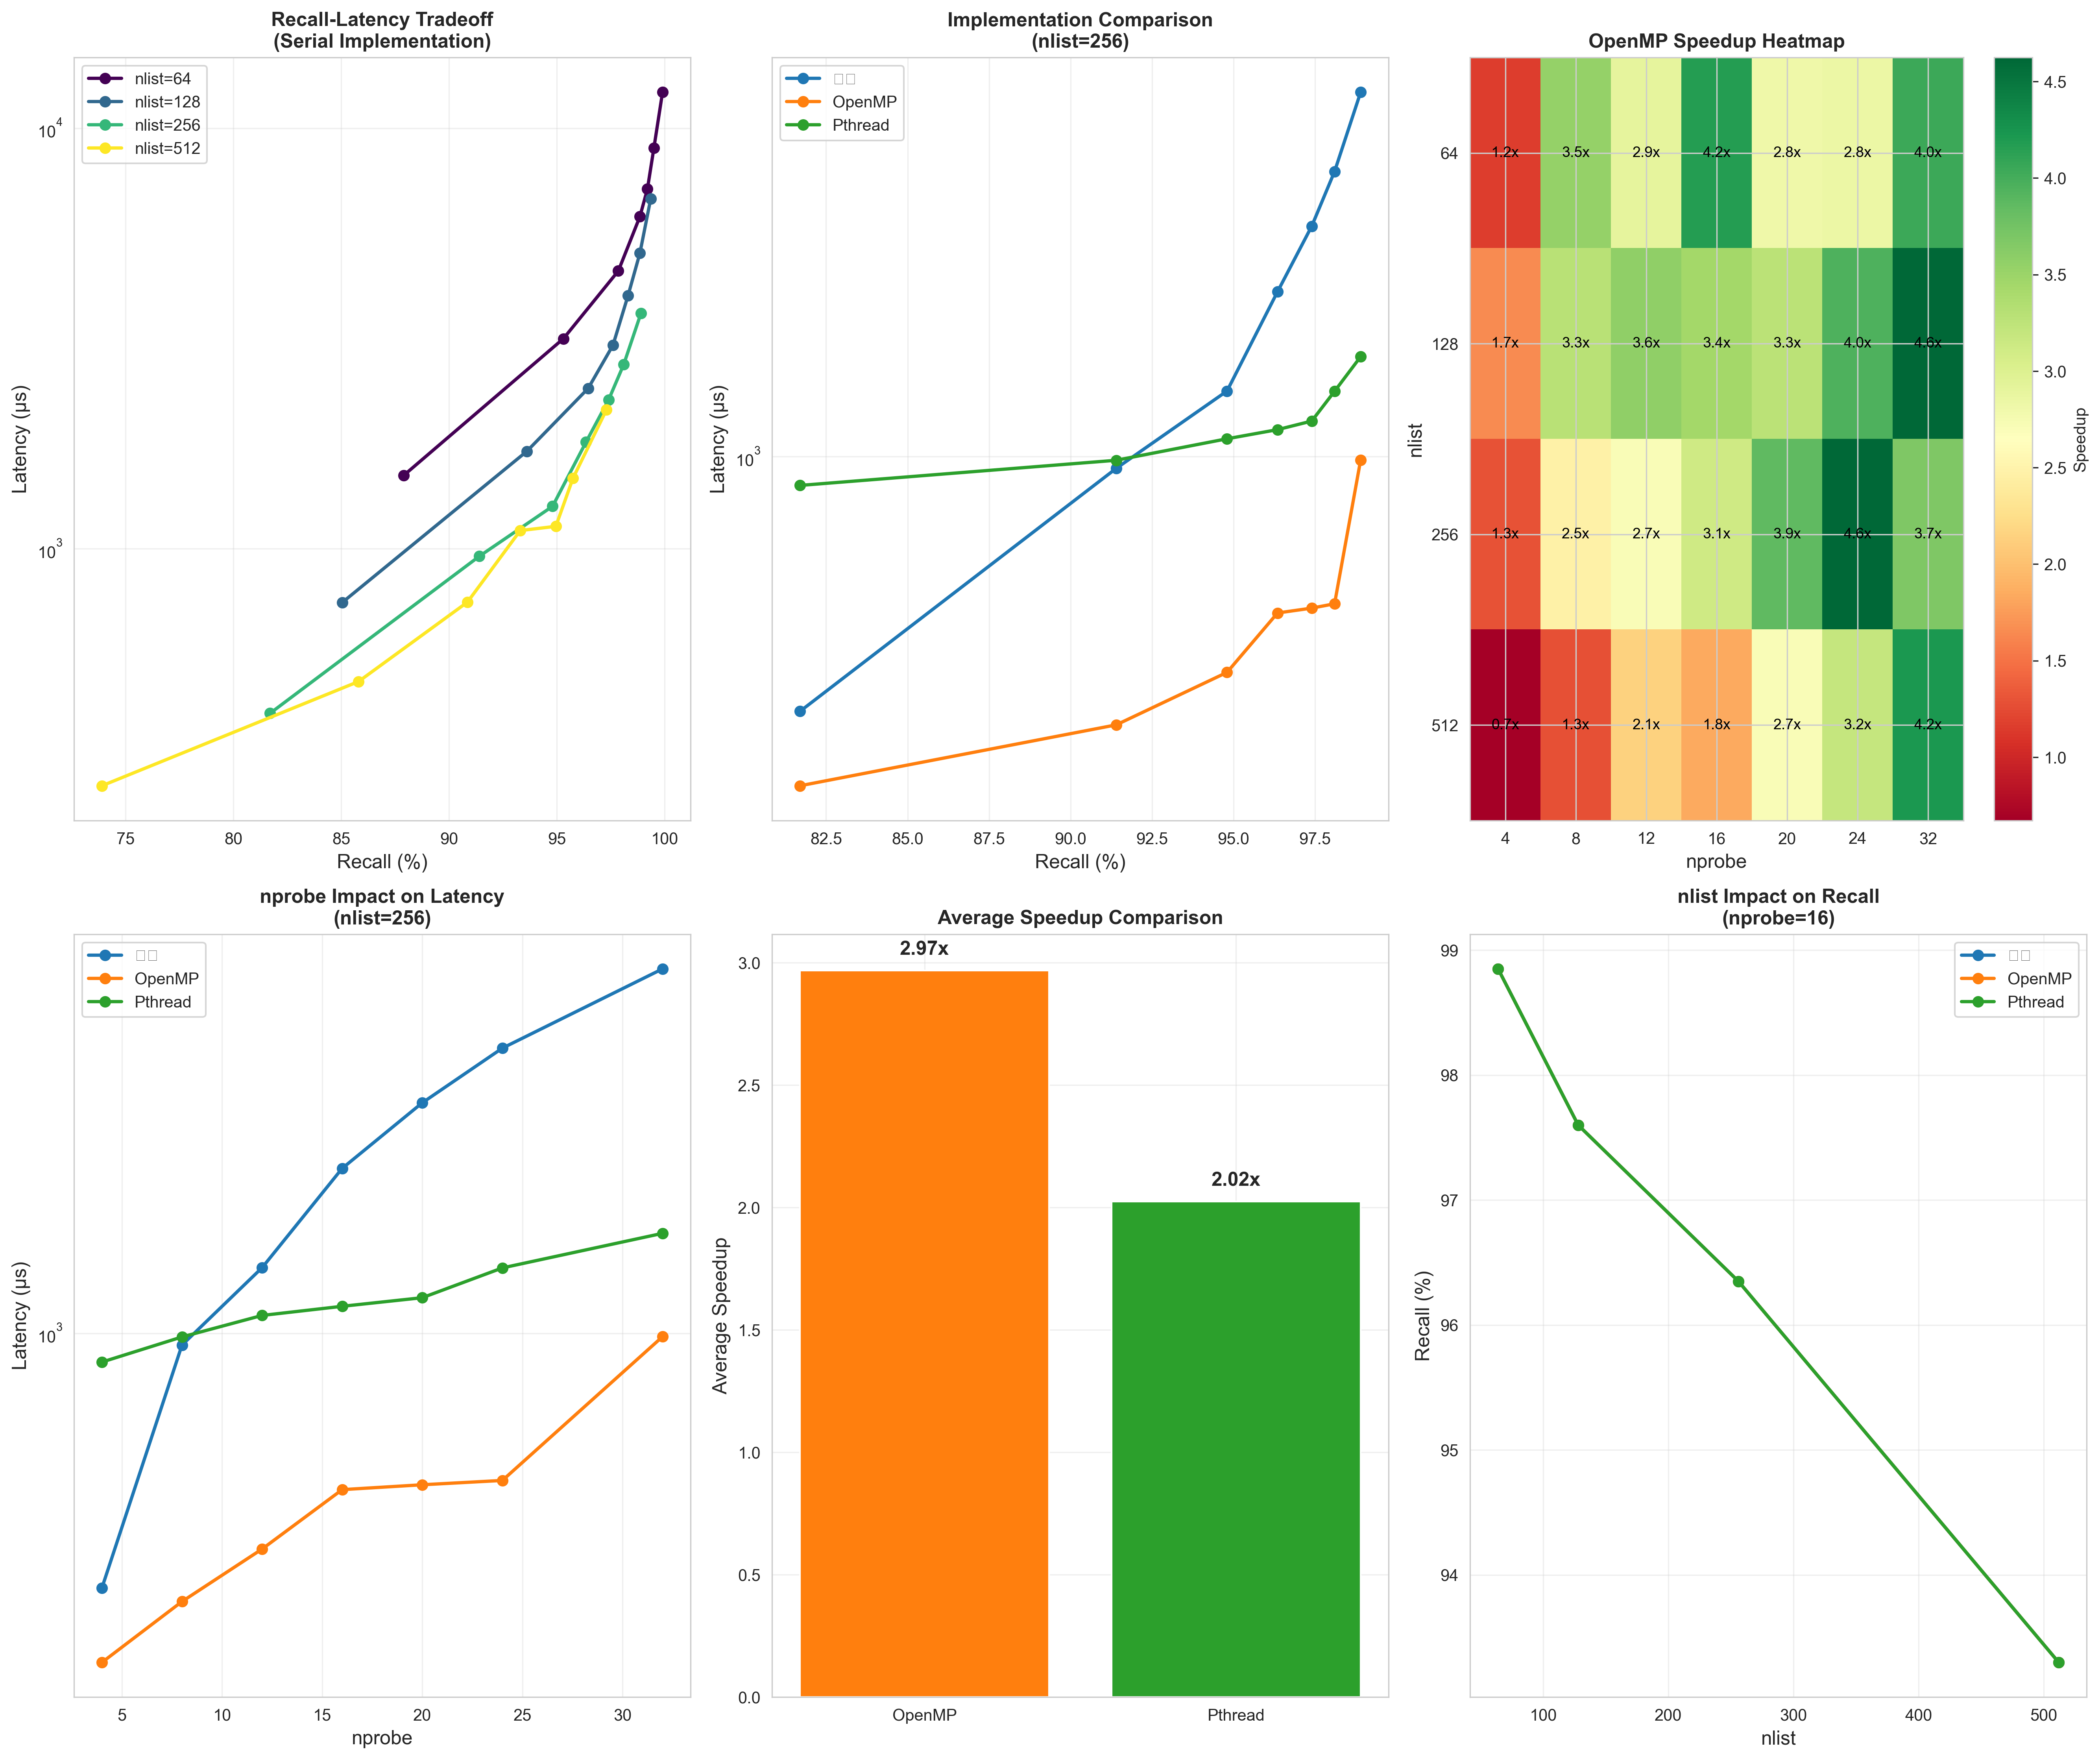
\includegraphics[width=\textwidth]{results/plots/ivf_comprehensive_analysis.png}
    \caption{IVF算法多线程实现综合性能分析}
    \label{fig:ivf_comprehensive}
\end{figure}

\textbf{1. 召回率-延迟权衡分析}

从图~\ref{fig:ivf_comprehensive}左上角的分析可以看出:
\begin{itemize}
    \item 随着nlist增大,在相同召回率下延迟显著降低
    \item nlist=512时能够以最低延迟达到较高召回率
    \item 存在明显的召回率-延迟权衡关系,nprobe增大时召回率提升但延迟增加
\end{itemize}

\textbf{2. 多线程实现效果比较}

对比三种实现方式在nlist=256配置下的性能(图~\ref{fig:ivf_comprehensive}右上角):
\begin{itemize}
    \item OpenMP实现在各召回率水平下均显示出最佳的延迟性能
    \item Pthread实现相比串行版本有明显改善,但不如OpenMP实现
    \item 在高召回率需求下,多线程优势更加明显
\end{itemize}

\textbf{3. 加速比分析}

表~\ref{tab:ivf_speedup_summary}总结了各实现的加速比统计:

\begin{table}[htbp]
    \centering
    \caption{IVF算法多线程实现加速比统计}
    \label{tab:ivf_speedup_summary}
    \begin{tabular}{lccc}
        \hline
        实现方式 & 平均加速比 & 最大加速比 & 最小加速比 \\
        \hline
        OpenMP & 2.97x & 4.62x & 0.67x \\
        Pthread & 2.02x & 4.58x & 0.31x \\
        \hline
    \end{tabular}
\end{table}

从热力图分析(图~\ref{fig:ivf_comprehensive}右中)可以观察到:
\begin{itemize}
    \item OpenMP实现在nlist=128, nprobe=32时达到最高加速比4.62x
    \item 加速比与参数配置密切相关,高nprobe值通常获得更好的加速效果
    \item 某些配置下加速比低于1.0,说明并行开销超过了并行收益
\end{itemize}

\paragraph{参数敏感性分析}

\textbf{1. nprobe参数影响}

图~\ref{fig:ivf_comprehensive}左下角显示了nprobe对延迟的影响:
\begin{itemize}
    \item 随着nprobe增加,延迟近似线性增长
    \item OpenMP实现在所有nprobe值下都保持最低延迟
    \item 并行化在高nprobe值时效果更加显著
\end{itemize}

\textbf{2. nlist参数影响}

图~\ref{fig:ivf_comprehensive}右下角分析了nlist对召回率的影响:
\begin{itemize}
    \item nlist从64增加到512时,召回率呈下降趋势
    \item 这是由于更多的聚类中心导致数据分布更分散
    \item 需要在召回率和计算效率之间找到平衡点
\end{itemize}

\paragraph{最优配置推荐}

基于实验结果,我们提出以下配置建议:

\textbf{高召回率场景}:
\begin{itemize}
    \item 推荐配置:nlist=64, nprobe=32, OpenMP实现
    \item 性能:召回率99.9\%,延迟3010μs,加速比4.04x
\end{itemize}

\textbf{低延迟场景}:
\begin{itemize}
    \item 推荐配置:nlist=256, nprobe=4, OpenMP实现
    \item 性能:召回率81.7\%,延迟312μs,加速比1.30x
\end{itemize}

\textbf{平衡场景}:
\begin{itemize}
    \item 推荐配置:nlist=256, nprobe=16, OpenMP实现
    \item 性能:召回率96.35\%,延迟575μs,加速比3.12x
\end{itemize}

\paragraph{多线程优化效果总结}

实验结果表明:
\begin{enumerate}
    \item OpenMP实现显著优于Pthread实现,平均加速比达到2.97x
    \item 并行化效果与参数配置强相关,高计算负载下并行收益更明显
    \item IVF算法具有良好的并行性,适合多线程优化
    \item 合理的参数选择对于实现高效的并行化至关重要
\end{enumerate}

这些结果为实际应用中的IVF算法参数调优和实现选择提供了重要参考。 